\documentclass[letterpaper,9pt,twocolumn,twoside,]{pinp}

%% Some pieces required from the pandoc template
\providecommand{\tightlist}{%
  \setlength{\itemsep}{0pt}\setlength{\parskip}{0pt}}

% Use the lineno option to display guide line numbers if required.
% Note that the use of elements such as single-column equations
% may affect the guide line number alignment.

\usepackage[T1]{fontenc}
\usepackage[utf8]{inputenc}

% pinp change: the geometry package layout settings need to be set here, not in pinp.cls
\geometry{layoutsize={0.95588\paperwidth,0.98864\paperheight},%
  layouthoffset=0.02206\paperwidth, layoutvoffset=0.00568\paperheight}

\definecolor{pinpblue}{HTML}{185FAF}  % imagecolorpicker on blue for new R logo
\definecolor{pnasbluetext}{RGB}{101,0,0} %


\usepackage{booktabs}
\usepackage{longtable}
\usepackage{array}
\usepackage{multirow}
\usepackage{wrapfig}
\usepackage{float}
\usepackage{colortbl}
\usepackage{pdflscape}
\usepackage{tabu}
\usepackage{threeparttable}
\usepackage{threeparttablex}
\usepackage[normalem]{ulem}
\usepackage{makecell}
\usepackage{xcolor}

\title{Modelling Body Fat Conveniently and Accurately}

\author[]{T09oc\_ontime\_1}

  \affil[]{The University of Sydney, Camperdown, NSW, 2006}

\setcounter{secnumdepth}{5}

% Please give the surname of the lead author for the running footer
\leadauthor{}

% Keywords are not mandatory, but authors are strongly encouraged to provide them. If provided, please include two to five keywords, separated by the pipe symbol, e.g:
 \keywords{  Regression |  Body fat density |  Model selection  }  

\begin{abstract}

\end{abstract}

\dates{A group project for the DATA2902 unit.}


% initially we use doi so keep for backwards compatibility
% new name is doi_footer

\pinpfootercontents{Modelling Body Fat Conveniently and Accurately}

\begin{document}

% Optional adjustment to line up main text (after abstract) of first page with line numbers, when using both lineno and twocolumn options.
% You should only change this length when you've finalised the article contents.
\verticaladjustment{-2pt}

\maketitle
\thispagestyle{firststyle}
\ifthenelse{\boolean{shortarticle}}{\ifthenelse{\boolean{singlecolumn}}{\abscontentformatted}{\abscontent}}{}

% If your first paragraph (i.e. with the \dropcap) contains a list environment (quote, quotation, theorem, definition, enumerate, itemize...), the line after the list may have some extra indentation. If this is the case, add \parshape=0 to the end of the list environment.


\hypertarget{abstract}{%
\section{Abstract}\label{abstract}}

Body fat percentage is a popular method of assessing an individual's
health. However, accurate measurements are inconvenient and costly.
Using a dataset collected in 1985, our group found two noteworthy models
for predicting body fat percentage; one more accurate that the other and
another more convenient. The more convenient uses four measurements:
weight and the circumferences of the abdomen, wrist and forearm.

\hypertarget{introduction}{%
\section{Introduction}\label{introduction}}

Body fat exists in two forms: essential body fat and storage body fat.
Essential body fat is required for survival, whereas storage body fat is
not. In high levels, storage body fat is a risk factor for various forms
of disease, such as type two diabetes and cardiovascular disease.
Knowing one's body fat percentage thus becomes important for maintaining
one's health.

Currently, one of the most accurate methods for measuring body fat is
retrieving one's underwater density. The underwater density measurement
is then used to estimate body fat percentage using Siri's equation:

\[
    PBF = \frac{495}{D} - 450
\] where \(PBF\) is the percentage of body fat and \(D\) is body density
in \(g/cm^3\).

Although relatively accurate, this method is both time consuming,
costly, and impractical for most individuals. Several alternatives have
been proposed, including weight, body mass index (BMI), and
circumference measurements of specific anatomical regions that
accumulate fat tissue. Although combining all these factors may give the
most accurate estimate of an individual's body fat percentage, it is not
the most practical: rather, a practical estimate should make use of a
limited number of factors that most people can calculate in their own
home. It is not yet clear from the literature which combination of
factors -- if any -- result in both a practical and accurate estimate of
an individual's body fat percentage.

In this report, we aimed to answer the following question: is there an
easy and accurate way to estimate one's body fat percentage?

To answer this question, we designed a multiple linear regression models
and assess them in terms of their practicality and performance. We
compare the performance of our model against the body fat measure
estimated by Siri's equation.

\hypertarget{data-set}{%
\section{Data set}\label{data-set}}

The data set \citep{dataset1985} consists 15 biometric measurements of
252 different men aged 22 to 81. It was collected in 1985 by the Human
Performance Research Center at Brigham Young University in Utah using a
central composite rotatable design sampling technique. This technique
was chosen because it is relatively robust and unbiased. The
measurements recorded include age, height, weight, body density, body
fat percentage and 10 circumference measurements of different anatomical
regions. Table \ref{ida:sum} shows summary statistics of the data set's
variables.

\hypertarget{data-cleaning}{%
\subsection{Data cleaning}\label{data-cleaning}}

As mentioned previously, a measure of underwater density is an
impractical for most people to obtain. Since we are concerned with
designing a convenient model, we chose to remove it from the set of
predictors in our data set.

\hypertarget{analysis}{%
\section{Analysis}\label{analysis}}

\hypertarget{pre-assumptions}{%
\subsection{Pre-Assumptions}\label{pre-assumptions}}

All predictors except height satisfied the linearity assumption (Figure
\ref{lin:o}). Because height did not satisfy this assumption (Figure
\ref{lin:h}), we removed it from our set of predictor variables. A
second assumption we must consider is that all observations between
groups and within groups are independent. Here, each observation in the
data corresponds to a unique male. This is a derivative of the study
design, notably the central composite rotatable sampling technique, and
means that the independence assumption must hold.

\hypertarget{model-selection}{%
\subsection{Model Selection}\label{model-selection}}

We used two methods for selecting viable models which estimate body fat
percentage. The first is the stepwise model selection process, in which
variables are removed from the full model or added from the null model
iteratively according to whether which variables improve the model's
accuracy score, as measured by the Akaike information criterion (AIC).

The variable inclusion plot visualises which variables are consistently
included in the best model as the penalty parameter, \(\lambda\),
changes. It shows that abdomen, wrist, forearm and neck circumference,
as well as weight and age, are stable contributors to the best models.
The remaining variables appear to stay within the vicinity of the random
variable labelled RV, which indicates they are of no predictive
significance (Figure \ref{mplot:inc}).

The model stability plot shows the probability that a model performs the
highest out of all the models at a given parameter size. This is
indicated by the bubble size, whilst the y-axis measures the degree of
error attributed to a model. We decided to choose the two most probable
models out of models of parameter size four and six, since they appear
to be simple and well performing (Figure \ref{mplot:stab}). From now on,
we refer to the four parameter and six parameter chosen models as the
``small'' and ``medium'' models respectively.

Two other models obtained from the forwards and backwards step-wise
selection procedures, alongside the coefficients for the small and
medium models are shown in table \ref{tab:mod}.

\hypertarget{post-assumptions}{%
\subsection{Post-Assumptions}\label{post-assumptions}}

For the four models obtained here, the homoscedasticity assumption is
satisfied (Figure \ref{homo:assum}), whilst the Central Limit Theorem
(CLT) and the sample size imply that the normality assumption isn't
violated.

\hypertarget{results}{%
\section{Results}\label{results}}

In considering the in-sample performance, measured using the R-squared
and AIC, the four models performed similarly as they were trained to fit
the sample. To compare the out-of-sample performance, we compared the
root mean square error (RMSE) (the difference between the predicted and
the real values), the mean absolute error (MAE) (a measure more robust
to outliers).

All models performed relatively similarly when comparing R-squared
values, RMSE, and MAE (Table \ref{results}).

\hypertarget{discussion-and-conclusion}{%
\section{Discussion and Conclusion}\label{discussion-and-conclusion}}

\hypertarget{interpretation-of-coefficients}{%
\subsection{Interpretation of
coefficients}\label{interpretation-of-coefficients}}

Our results showed that the four models had similar in-sample and
out-of-sample performance. The main differences in the models are the
number of parameters included. In this respect, the four parameter model
is selected as the final model because it is the simplest.

The equation for the final model is, \[
\begin{aligned}
\operatorname{\widehat{Fat}} &= -34.85 + 1(\operatorname{Abdomen}) - 0.3(\operatorname{Weight}) - 1.51(\operatorname{Wrist})\ + \\
&\quad 0.47(\operatorname{Forearm})
\end{aligned}
\]

This equation predicts that a one percent increase in body fat
percentage results in the following changes to the predictor variables:

\begin{itemize}
\tightlist
\item
  A 10 millimeter increase in abdomen circumference
\item
  A 300 gram decrease in weight
\item
  A 15 millimeter decrease in wrist circumference
\item
  A 5 millimeter increase in forearm circumference
\end{itemize}

Increases in abdomen circumference align with what we would expect for
an increase in body fat percentage: men typically accumulate adipose
tissue around their abdomen \citep{heitmann1991body}. Increases in
forearm circumference have also been reported
\citep{haffner1993obesity}. Interestingly, our model suggests that an
increase in body fat percentage is also associated with a decrease in
weight and wrist circumference. These results do not align with what has
been reported in existing obesity literature \citep{haffner1993obesity};
\citep{heitmann1991body}. One possible explanation for this discrepency
is that body fat percentage was overestimated for older participants in
our study. The Siri equation, which is the estimate of body fat
percentage used in this study, has been reported to over estimate body
fat percentage for individuals above sixty years old
\citep{guerra2010accuracy}. In our study cohort, fourteen percent of
participants were aged above sixty. The overestimate of body fat that
occurred for elderly participants would also explain the negative
coefficients for wrist circumference and weight, because weight and bone
density decrease with age.

One opportunity for future work in this area would be to investigate
which variables are most important and predictive of body fat percentage
when body fat is estimated using a measure that does not overestimate
for elderly individuals, such as dry electrode-based body fat
estimation.

To conclude, we set out to determine whether there is an easy and
accurate way to estimate one's body fat percentage. We obtained a model
that requires only four measurements and is reasonably accurate. One
limitation of this study was that the body fat estimate used may have
overestimated for elderly participants, subsequently affecting the
coefficients in our model. Future work should investigate whether these
coefficients change when we use a more accurate estimate of body fat
percentage.

\hypertarget{appendix}{%
\section{Appendix}\label{appendix}}

See overleaf figures and tables that could not be condensed into the
executive summary.

\begin{table}

\caption{\label{tab:unnamed-chunk-4}\label{ida:sum} \textnormal{A table with summary statistics of the data set.}}
\centering
\begin{tabular}[t]{l|r|r|r}
\hline
  & Min & Max & Mean\\
\hline
Underwater Density (gm/cm\textasciicircum{}3) & 1.0 & 1.1 & 1.1\\
\hline
Fat (\%) & 0.0 & 47.5 & 19.2\\
\hline
Age (years) & 22.0 & 81.0 & 44.9\\
\hline
Height (cm) & 74.9 & 197.5 & 178.2\\
\hline
Weight (kg) & 53.8 & 164.7 & 81.2\\
\hline
Neck (cm) & 31.1 & 51.2 & 38.0\\
\hline
Chest (cm) & 79.3 & 136.2 & 100.8\\
\hline
Abdomen (cm) & 69.4 & 148.1 & 92.6\\
\hline
Hip (cm) & 85.0 & 147.7 & 99.9\\
\hline
Thigh (cm) & 47.2 & 87.3 & 59.4\\
\hline
Knee (cm) & 33.0 & 49.1 & 38.6\\
\hline
Ankle (cm) & 19.1 & 33.9 & 23.1\\
\hline
Bicep (cm) & 24.8 & 45.0 & 32.3\\
\hline
Forearm (cm) & 21.0 & 34.9 & 28.7\\
\hline
Wrist (cm) & 15.8 & 21.4 & 18.2\\
\hline
\end{tabular}
\end{table}

\begin{figure}

{\centering 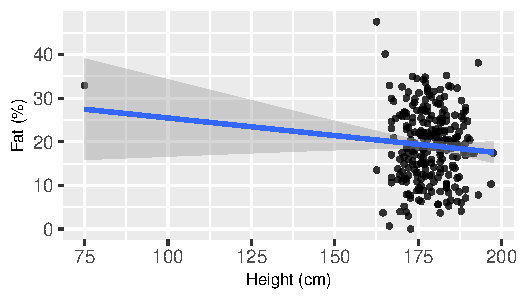
\includegraphics{template_report_files/figure-latex/linear-height-1} 

}

\caption{\label{lin:h} A scatter plot with fitted linear model of body fat percentage versus height.}\label{fig:linear-height}
\end{figure}

\begin{figure}

{\centering 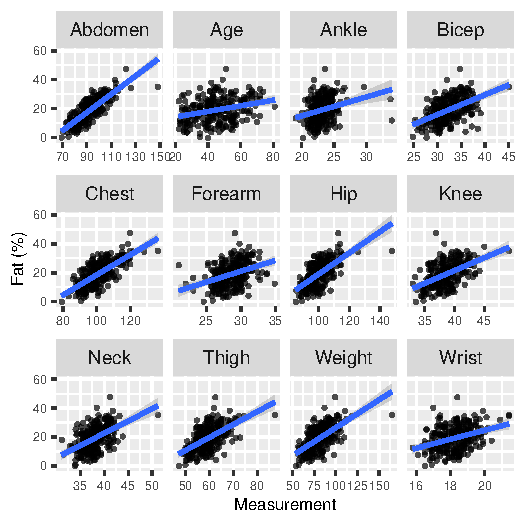
\includegraphics{template_report_files/figure-latex/linear-other-1} 

}

\caption{\label{lin:o} A scatter plot for each predictor which observe a linear relationship with body fat.}\label{fig:linear-other}
\end{figure}

\begin{figure}

{\centering 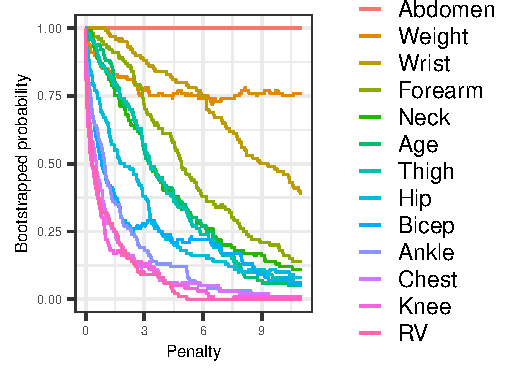
\includegraphics{template_report_files/figure-latex/unnamed-chunk-5-1} 

}

\caption{\label{mplot:inc} Each variable's probability of inclusion in the best model as it's penalty varies.}\label{fig:unnamed-chunk-5}
\end{figure}

\begin{figure}

{\centering 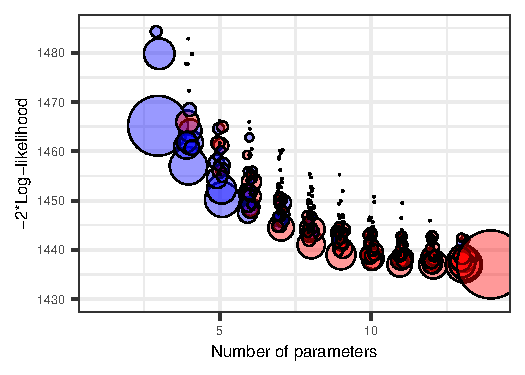
\includegraphics{template_report_files/figure-latex/unnamed-chunk-6-1} 

}

\caption{\label{mplot:stab} Stability of every possible model as the number parameters change. The size of the circle indicates the probability of being selected as the best model.}\label{fig:unnamed-chunk-6}
\end{figure}

\begin{table}[!htbp] \centering 
  \caption{\textnormal{Table summary of the four selected models.}} 
  \label{tab:mod} 
\begin{tabular}{@{\extracolsep{5pt}}lcccc} 
\\[-1.8ex]\hline 
\hline \\[-1.8ex] 
 & \multicolumn{4}{c}{\textit{Dependent variable:}} \\ 
\cline{2-5} 
\\[-1.8ex] & \multicolumn{4}{c}{Fat} \\ 
 & Fowards Step & Backwards Step & Small & Medium \\ 
\\[-1.8ex] & (1) & (2) & (3) & (4)\\ 
\hline \\[-1.8ex] 
 Age & 0.06$^{*}$ & 0.07$^{**}$ &  & 0.06$^{**}$ \\ 
  Height & $-$0.03 &  &  &  \\ 
  Weight & $-$0.19$^{*}$ & $-$0.20$^{**}$ & $-$0.30$^{***}$ & $-$0.30$^{***}$ \\ 
  Neck & $-$0.47$^{**}$ & $-$0.47$^{**}$ &  &  \\ 
  Chest & $-$0.02 &  &  &  \\ 
  Abdomen & 0.95$^{***}$ & 0.94$^{***}$ & 1.00$^{***}$ & 0.91$^{***}$ \\ 
  Hip & $-$0.21 & $-$0.20 &  &  \\ 
  Thigh & 0.24 & 0.30$^{**}$ &  & 0.22$^{*}$ \\ 
  Knee & 0.02 &  &  &  \\ 
  Ankle & 0.17 &  &  &  \\ 
  Bicep & 0.18 &  &  &  \\ 
  Forearm & 0.45$^{**}$ & 0.52$^{***}$ & 0.47$^{***}$ & 0.49$^{***}$ \\ 
  Wrist & $-$1.62$^{***}$ & $-$1.54$^{***}$ & $-$1.51$^{***}$ & $-$1.78$^{***}$ \\ 
  Constant & $-$18.19 & $-$22.66$^{*}$ & $-$34.85$^{***}$ & $-$38.32$^{***}$ \\ 
 \hline \\[-1.8ex] 
R$^{2}$ & 0.75 & 0.75 & 0.74 & 0.74 \\ 
Adjusted R$^{2}$ & 0.74 & 0.74 & 0.73 & 0.73 \\ 
\hline 
\hline \\[-1.8ex] 
\textit{Note:}  & \multicolumn{4}{r}{$^{*}$p$<$0.1; $^{**}$p$<$0.05; $^{***}$p$<$0.01} \\ 
\end{tabular} 
\end{table}

\begin{figure}

{\centering 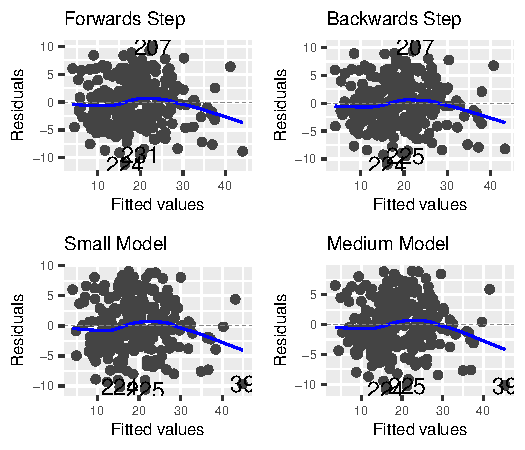
\includegraphics{template_report_files/figure-latex/assump-homo-1} 

}

\caption{\label{homo:assum} Residuals of each model against the fitted values. This a a check for homoscedasticity by checking for equal spread of the residuals.}\label{fig:assump-homo}
\end{figure}

\graphicspath{ {./} }
\begin{figure}
    \caption{\label{results} Table of the in-sample and out of sample results for each model.}
    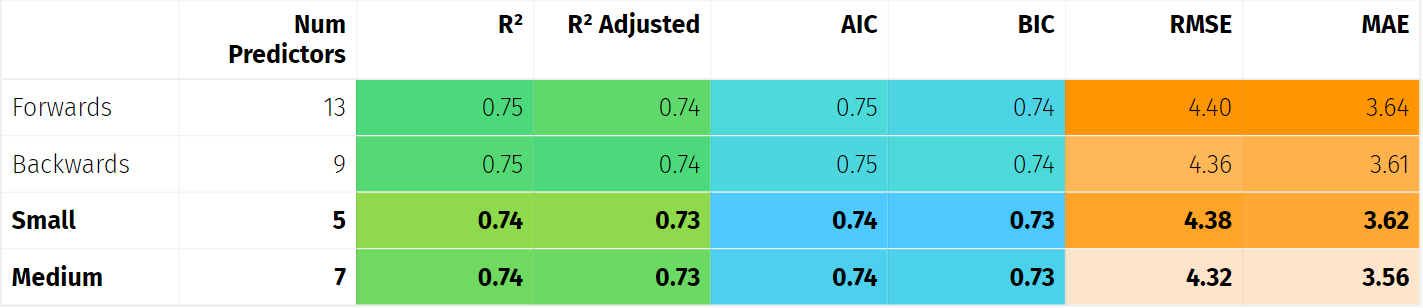
\includegraphics[scale=0.3]{results.png}
\end{figure}

%\showmatmethods


\bibliography{pinp}
\bibliographystyle{jss}



\end{document}
